% Boundra security self-assessment report. Compile with Tectonic: tectonic -X compile security-assessment.tex
\documentclass[11pt,a4paper,oneside]{report}
% Shared Boundra document style: fonts, brand colours, headings, callouts, tables, diagrams.
% Used by boundra-technical.tex, security-assessment.tex and execution-evidence.tex.

% ---------------------------------------------------------------- Page and fonts
\usepackage[a4paper,left=2.3cm,right=2.3cm,top=2.6cm,bottom=2.4cm,headheight=14pt]{geometry}
\usepackage{fontspec}
\setmainfont{Inter}[Extension=.otf,UprightFont=*-Regular,BoldFont=*-SemiBold,
  ItalicFont=*-Italic,BoldItalicFont=*-SemiBoldItalic,Scale=0.92]
\newfontfamily\headfont{SourceSerifPro}[Extension=.otf,UprightFont=*-Semibold,
  BoldFont=*-Bold,ItalicFont=*-SemiboldIt]
\setmonofont{SourceCodePro}[Extension=.otf,UprightFont=*-Regular,BoldFont=*-Semibold,Scale=0.86]
\linespread{1.12}
\setlength{\parindent}{0pt}
\setlength{\parskip}{0.55em}
\usepackage{microtype}
\usepackage{placeins}
\setlength{\emergencystretch}{3em}

% ---------------------------------------------------------------- Brand colours (apps/web/src/app/globals.css)
\usepackage{xcolor}
\definecolor{bForest}{HTML}{122D27}
\definecolor{bGreen}{HTML}{23674E}
\definecolor{bIvory}{HTML}{F6F8F2}
\definecolor{bSage}{HTML}{9BAF8D}
\definecolor{bLime}{HTML}{A6C74C}
\definecolor{bAmber}{HTML}{D8A13B}
\definecolor{bCharcoal}{HTML}{19332D}
\definecolor{bMuted}{HTML}{4D6058}
\definecolor{bMutedDark}{HTML}{B8C7BB}
\definecolor{bSurface}{HTML}{FCFDF9}
\definecolor{bSageSoft}{HTML}{E4EBDA}
\definecolor{bLimeSoft}{HTML}{E1ECBF}
\definecolor{bAmberSoft}{HTML}{F7E9CB}
\definecolor{bAmberInk}{HTML}{8A5A0B}
\definecolor{bLine}{HTML}{D3D9D2}
\color{bForest}

% ---------------------------------------------------------------- Packages
\usepackage{tikz}
\usetikzlibrary{svg.path,positioning,arrows.meta,shapes.geometric,fit,backgrounds,calc,shadows}
\usepackage[most]{tcolorbox}
\usepackage{booktabs,tabularx,xltabular,array,colortbl,multirow}
\usepackage{enumitem}
\usepackage{titlesec,titletoc}
\usepackage{fancyhdr}
\usepackage{listings}
\usepackage{amsmath}
\usepackage[hidelinks]{hyperref}
\hypersetup{pdftitle={Boundra: Technical Document},pdfauthor={Boundra team},
  colorlinks=true,linkcolor=bGreen,urlcolor=bGreen}

% ---------------------------------------------------------------- Headings
\titleformat{\chapter}[display]
  {\headfont\color{bForest}}
  {\normalfont\small\bfseries\color{bGreen}\MakeUppercase{Chapter}~\thechapter}
  {4pt}
  {\Huge}
  [\vspace{4pt}{\color{bLime}\rule{2.2cm}{2.5pt}}]
\titlespacing*{\chapter}{0pt}{-12pt}{18pt}
% A heading always keeps a few lines of its section with it on the page.
\titleformat{\section}{\headfont\Large\color{bForest}}{\color{bGreen}\thesection}{0.7em}{}
\titlespacing*{\section}{0pt}{1.4em}{0.5em}
\titleformat{\subsection}{\headfont\large\color{bForest}}{\color{bGreen}\thesubsection}{0.6em}{}
\titlespacing*{\subsection}{0pt}{1.1em}{0.35em}
\titleformat{\paragraph}[runin]{\bfseries\color{bForest}}{}{}{}[.]
\titlespacing*{\paragraph}{0pt}{0.5em}{0.6em}
\setcounter{secnumdepth}{2}
\setcounter{tocdepth}{1}

% Table of contents
\titlecontents{chapter}[2.2em]{\addvspace{0.42em}\headfont}
  {\contentslabel[\color{bGreen}\thecontentslabel]{2.2em}}{}{\hfill\contentspage}
\titlecontents{section}[4.8em]{\small}
  {\contentslabel[\color{bMuted}\thecontentslabel]{2.6em}}{}
  {\titlerule*[0.6pc]{\color{bLine}.}\contentspage}

% ---------------------------------------------------------------- Header and footer
\pagestyle{fancy}
\fancyhf{}
\renewcommand{\chaptermark}[1]{\markboth{#1}{}}
% Each document sets its own name with \renewcommand{\docname}{...} after loading this style.
\newcommand{\docname}{Technical document}
\fancyhead[L]{\small\color{bMuted}\brandmark[0.17]\hspace{0.45em}Boundra\,·\,\docname}
\fancyhead[R]{\small\color{bMuted}\nouppercase{\leftmark}}
\fancyfoot[R]{\small\color{bGreen}\bfseries\thepage}
\fancyfoot[L]{\small\color{bMuted}Base Sepolia testnet prototype\,·\,no real funds}
\renewcommand{\headrule}{{\color{bLine}\hrule height 0.5pt}}
\fancypagestyle{plain}{\fancyhf{}\renewcommand{\headrule}{}
  \fancyfoot[R]{\small\color{bGreen}\bfseries\thepage}}

% ---------------------------------------------------------------- Lists
\setlist{itemsep=0.15em,topsep=0.25em,parsep=0.1em}
\setlist[itemize,1]{label={\color{bLime}\rule[0.18em]{0.42em}{0.42em}},leftmargin=1.3em}
\setlist[itemize,2]{label={\color{bSage}\textbullet},leftmargin=1.2em}
\setlist[enumerate,1]{label={\color{bGreen}\bfseries\arabic*.},leftmargin=1.6em}

% ---------------------------------------------------------------- Brand mark (apps/web/src/components/brand-mark.tsx)
\newcommand{\markforest}{svg{M9.4 9.7C8.6 10.5 7.3 12 6.3 13.2C5.4 14.5 4.6 15.9 3.8 17.2C3.1 18.5 2.4 19.8 1.9 21.2C1.3 22.6 0.9 24.1 0.5 25.6C0.2 27.1 0.1 28.6 0 30.1C-0.1 31.6 0 33.2 0.2 34.7C0.4 36.2 0.7 37.8 1.1 39.2C1.5 40.7 2 42.1 2.7 43.5C3.3 44.9 4 46.3 4.8 47.6C5.6 48.8 6.5 50.1 7.5 51.2C8.5 52.4 9.6 53.5 10.8 54.4C11.9 55.4 13.1 56.3 14.4 57.2C15.6 58 16.9 58.7 18.3 59.3C19.6 59.9 21 60.5 22.4 60.9C23.8 61.4 25.3 61.8 26.9 62C28.4 62.2 30.1 62.4 31.6 62.3C33.2 62.2 34.9 61.9 36.3 61.4C37.8 61 39.2 60.4 40.5 59.8C41.8 59.1 43.1 58.4 44.2 57.6C45.3 56.8 46.4 55.9 47.4 55C48.4 54.1 49.3 53.1 50.1 52.1C51 51.1 51.8 50 52.3 49.2C52.8 48.4 53.2 47.9 53.3 47.2C53.5 46.5 53.4 45.6 53.2 44.9C53 44.2 52.5 43.5 51.9 43C51.4 42.5 50.6 42.2 49.9 42C49.2 41.9 48.3 41.9 47.6 42.2C47 42.4 46.4 42.8 45.8 43.4C45.1 44 44.3 44.9 43.6 45.5C42.8 46.1 42 46.5 41.3 47C40.5 47.4 39.6 47.8 38.8 48.1C38 48.4 37.1 48.7 36.3 48.9C35.4 49.1 34.6 49.3 33.8 49.3C33 49.4 32.3 49.4 31.5 49.3C30.8 49.2 30 49.1 29.3 48.9C28.5 48.7 27.7 48.4 27 48.1C26.2 47.8 25.4 47.4 24.7 46.9C23.9 46.5 23.2 46 22.6 45.5C21.9 44.9 21.3 44.4 20.8 43.8C20.2 43.2 19.7 42.5 19.2 41.9C18.8 41.2 18.4 40.5 18 39.8C17.6 39 17.3 38.3 17 37.5C16.7 36.7 16.4 35.9 16.2 35.1C16 34.3 15.9 33.5 15.7 32.7C15.6 31.8 15.5 31 15.5 30.1C15.4 29.2 15.4 28.3 15.4 27.3C15.4 26.4 15.3 25.5 15.3 24.4C15.4 23.4 15.6 22.3 15.7 21.1C15.7 20 15.6 18.7 15.8 17.5C16 16.2 16.5 14.7 16.7 13.7C17 12.7 17.3 12.3 17.3 11.6C17.2 10.9 17 10.1 16.6 9.5C16.3 8.9 15.7 8.4 15.1 8C14.5 7.7 13.7 7.5 13 7.5C12.3 7.5 11.5 7.8 10.9 8.1C10.3 8.5 10.2 8.8 9.4 9.7Z}}
\newcommand{\marksage}{svg{M26.2 9.5C26.9 9.5 27.8 9.3 28.5 9.2C29.2 9.1 29.9 9.1 30.6 9.1C31.3 9.2 32 9.2 32.7 9.3C33.4 9.4 34 9.5 34.7 9.7C35.4 9.8 36 10 36.7 10.2C37.3 10.4 38 10.6 38.6 10.9C39.2 11.1 39.9 11.4 40.5 11.7C41.1 12 41.7 12.3 42.2 12.6C42.8 13 43.4 13.3 43.9 13.7C44.4 14.1 45 14.5 45.5 14.9C46 15.4 46.5 15.8 46.9 16.3C47.4 16.7 47.8 17.2 48.3 17.7C48.7 18.2 49.1 18.7 49.5 19.3C49.9 19.8 50.2 20.3 50.6 20.9C50.9 21.4 51.3 22 51.6 22.6C51.9 23.1 52.2 23.7 52.5 24.3C52.8 24.9 53.1 25.6 53.3 26.2C53.5 26.8 53.8 27.5 54 28.1C54.1 28.8 54.3 29.4 54.4 30.1C54.6 30.8 54.7 31.5 54.7 32.2C54.8 32.9 54.8 33.5 54.8 34.3C54.7 35 54.6 35.8 54.6 36.5C54.6 37.2 54.5 37.9 54.8 38.5C55 39.1 55.4 39.7 55.9 40.1C56.4 40.5 57.1 40.8 57.7 40.9C58.4 41 59.1 40.9 59.7 40.7C60.3 40.4 60.9 40 61.3 39.5C61.7 39 61.8 38.4 62.1 37.7C62.3 37 62.4 36 62.6 35.1C62.7 34.2 62.9 33.3 63 32.3C63.1 31.4 63.1 30.5 63.1 29.5C63.1 28.6 63.1 27.6 63 26.6C63 25.7 62.9 24.7 62.7 23.8C62.5 22.8 62.3 21.8 62 20.9C61.8 20 61.4 19 61.1 18.1C60.7 17.2 60.3 16.3 59.8 15.5C59.3 14.6 58.8 13.8 58.2 13C57.6 12.2 57 11.4 56.3 10.6C55.7 9.9 55 9.2 54.3 8.5C53.5 7.9 52.8 7.2 52 6.7C51.2 6.1 50.4 5.5 49.5 5C48.7 4.5 47.8 4 47 3.6C46.1 3.2 45.2 2.8 44.3 2.5C43.4 2.1 42.4 1.8 41.5 1.6C40.6 1.3 39.6 1.1 38.7 1C37.7 0.9 36.7 0.8 35.8 0.7C34.8 0.7 33.9 0.7 32.9 0.7C32 0.8 31 0.9 30.1 1C29.1 1.1 28.2 1.3 27.3 1.4C26.4 1.6 25.4 1.8 24.7 2.1C24 2.3 23.4 2.5 23 3C22.5 3.4 22.1 4 21.9 4.6C21.7 5.2 21.6 5.9 21.7 6.6C21.9 7.2 22.2 7.8 22.6 8.3C23 8.8 23.7 9.2 24.3 9.4C24.9 9.6 25.5 9.6 26.2 9.5Z}}
% \brandmarkcol[scale]{outer colour}: the mark on its 64-unit grid (1 unit = 1pt at scale 1),
% with the forest arc in the given colour. \brandmark[scale] is the light-surface version.
\newcommand{\brandmarkcol}[2][1]{\begin{tikzpicture}[scale=#1,yscale=-1,
  baseline={([yshift=-1.2pt]current bounding box.south)}]
  \fill[#2] \markforest;
  \fill[bSage] \marksage;
  \fill[bLime] (32pt,32pt) circle (8.4pt);
\end{tikzpicture}}
\newcommand{\brandmark}[1][1]{\brandmarkcol[#1]{bForest}}

% ---------------------------------------------------------------- Callout boxes
\tcbset{boundra/.style={enhanced,boxrule=0pt,arc=3pt,left=10pt,right=10pt,
  top=7pt,bottom=7pt,fonttitle=\bfseries\small,coltitle=bForest,attach title to upper,
  before skip=0.9em,after skip=0.9em}}
\newtcolorbox{keypoint}[1][Key point]{boundra,colback=bLimeSoft,
  borderline west={3pt}{0pt}{bGreen},title={#1.\ }}
\newtcolorbox{note}[1][Note]{boundra,colback=bSageSoft,
  borderline west={3pt}{0pt}{bSage},title={#1.\ }}
\newtcolorbox{caution}[1][Caution]{boundra,colback=bAmberSoft,coltitle=bAmberInk,
  borderline west={3pt}{0pt}{bAmber},title={#1.\ }}
\newtcolorbox{principle}[1]{enhanced,boxrule=0pt,arc=4pt,colback=bForest,
  coltext=bIvory,left=12pt,right=12pt,top=9pt,bottom=9pt,fonttitle=\headfont\large,
  coltitle=bLime,title={#1},attach title to upper={\par\vspace{3pt}},before skip=1em,after skip=1em}

% ---------------------------------------------------------------- Tables
\newcolumntype{L}{>{\raggedright\arraybackslash}X}
\newcolumntype{P}[1]{>{\raggedright\arraybackslash}p{#1}}
\renewcommand{\arraystretch}{1.28}
\setlength{\tabcolsep}{5pt}
\arrayrulecolor{bSage}
\newcommand{\thead}[1]{\textbf{\color{bForest}#1}}
\newcommand{\headrow}{\rowcolor{bSageSoft}}
% Tables break across pages (xltabular = longtable + X columns) instead of leaving gaps.
\setlength{\LTleft}{0pt}
\setlength{\LTright}{0pt}
\setlength{\LTpre}{0pt}
\setlength{\LTpost}{0.4em}
% A table never starts on a new page away from the heading or text just above it.
\newenvironment{btable}[1]
  {\par\nopagebreak\vspace{0.6em}\small\xltabular{\linewidth}{#1}\toprule}
  {\bottomrule\endxltabular\par}
% Short tables (up to about eight rows) never split; they move with the heading or text above.
\newenvironment{stable}[1]
  {\par\nopagebreak\vspace{0.6em}\small\noindent\tabularx{\linewidth}{#1}\toprule}
  {\bottomrule\endtabularx\par\vspace{0.4em}}

% Floats: allow them close to their text, and top-align pages that hold only floats.
\renewcommand{\topfraction}{0.9}
\renewcommand{\bottomfraction}{0.8}
\renewcommand{\textfraction}{0.08}
\renewcommand{\floatpagefraction}{0.8}
\makeatletter
\setlength{\@fptop}{0pt}
\makeatother

% ---------------------------------------------------------------- Code and inline helpers
\lstdefinestyle{boundra}{basicstyle=\ttfamily\small\color{bForest},backgroundcolor=\color{bSurface},
  frame=single,rulecolor=\color{bLine},framesep=6pt,xleftmargin=6pt,xrightmargin=6pt,
  keywordstyle=\color{bGreen}\bfseries,commentstyle=\color{bMuted}\itshape,
  stringstyle=\color{bAmberInk},columns=fullflexible,keepspaces=true,breaklines=true,
  showstringspaces=false,aboveskip=0.8em,belowskip=0.6em}
\lstset{style=boundra}
\newcommand{\code}[1]{\texttt{\color{bGreen}#1}}
% Inside dark diagram boxes, code takes the box's text colour instead of green.
\newcommand{\plaincode}{\renewcommand{\code}[1]{\texttt{##1}}}
\newcommand{\term}[1]{\textbf{#1}}
\newcommand{\muted}[1]{{\color{bMuted}#1}}

% ---------------------------------------------------------------- Diagram styles
\tikzset{
  box/.style={draw=bForest,line width=0.6pt,rounded corners=3pt,fill=white,align=center,
    font=\small,inner sep=5pt,minimum height=9mm,text=bForest,
    execute at begin node={\hyphenpenalty=10000\exhyphenpenalty=10000}},
  % On dark fills, code takes the box's text colour instead of green.
  boxdark/.style={box,fill=bForest,text=bIvory,draw=bForest,
    execute at begin node={\hyphenpenalty=10000\exhyphenpenalty=10000\plaincode}},
  boxgreen/.style={box,fill=bGreen,text=white,draw=bGreen,
    execute at begin node={\hyphenpenalty=10000\exhyphenpenalty=10000\plaincode}},
  boxlime/.style={box,fill=bLimeSoft},
  boxsage/.style={box,fill=bSageSoft},
  boxamber/.style={box,fill=bAmberSoft,draw=bAmberInk},
  boxghost/.style={box,draw=bSage,dashed,text=bMuted},
  arr/.style={-{Stealth[length=2.2mm,width=1.8mm]},line width=0.65pt,draw=bGreen},
  arrm/.style={arr,draw=bMuted},
  arrd/.style={arr,dashed,draw=bMuted},
  arra/.style={arr,draw=bAmberInk},
  biarr/.style={{Stealth[length=2.2mm,width=1.8mm]}-{Stealth[length=2.2mm,width=1.8mm]},
    line width=0.65pt,draw=bGreen},
  lbl/.style={font=\scriptsize,text=bMuted,fill=white,inner sep=1.5pt,align=center},
  lblc/.style={font=\scriptsize,text=bMuted,inner sep=1.5pt,align=center},
  zone/.style={draw=bSage,line width=0.6pt,dashed,rounded corners=6pt,inner sep=9pt},
  zonefill/.style={fill=bSurface,draw=bSage,line width=0.6pt,rounded corners=6pt,inner sep=9pt},
  zonetitle/.style={font=\scriptsize\bfseries,text=bGreen,fill=white,inner sep=2pt},
  state/.style={draw=bForest,line width=0.6pt,rounded corners=7pt,fill=white,font=\scriptsize\ttfamily,
    inner sep=4pt,minimum height=7mm,text=bForest},
  stateok/.style={state,fill=bLimeSoft},
  statebad/.style={state,fill=bAmberSoft,draw=bAmberInk},
  statedone/.style={state,fill=bSageSoft},
  stepdot/.style={circle,fill=bGreen,text=white,font=\scriptsize\bfseries,inner sep=1.4pt,minimum size=4.6mm},
}
\newcommand{\stepno}[1]{\tikz[baseline=-0.6ex]\node[stepdot]{#1};}

\newcommand{\figcaption}[1]{\par\vspace{0.3em}{\centering\small\color{bMuted}#1\par}\vspace{0.6em}}


\renewcommand{\docname}{Security self-assessment}
\hypersetup{pdftitle={Boundra: Security Self-Assessment Report}}
% A short report: sections are the top level, numbered 1, 2, 3.
\renewcommand{\thesection}{\arabic{section}}
\renewcommand{\sectionmark}[1]{\markboth{#1}{}}
\titlecontents{section}[2.2em]{\addvspace{0.42em}\headfont}
  {\contentslabel[\color{bGreen}\thecontentslabel]{2.2em}}{}{\hfill\contentspage}
\titlecontents{subsection}[4.8em]{\small}
  {\contentslabel[\color{bMuted}\thecontentslabel]{2.6em}}{}
  {\titlerule*[0.6pc]{\color{bLine}.}\contentspage}
\setcounter{tocdepth}{2}
\newcommand{\yes}{{\color{bGreen}\textbf{yes}}}
\newcommand{\no}{{\color{bMuted}no}}
\newcommand{\impact}[1]{\textbf{#1}}

\begin{document}

\begin{titlepage}
\thispagestyle{empty}

\begin{tikzpicture}[remember picture,overlay]
  \fill[bForest] (current page.south west) rectangle (current page.north east);
  \draw[bGreen,line width=26pt,opacity=0.35]
    ($(current page.south east)+(-2.2,6.5)$) arc[start angle=-10,end angle=120,radius=9.5];
  \draw[bLime,line width=3pt,opacity=0.55]
    ($(current page.south east)+(-1.2,4.6)$) arc[start angle=-20,end angle=95,radius=7.2];
  \node[anchor=north west,inner sep=0] at ($(current page.north west)+(2.3,-2.6)$)
    {\brandmarkcol[1.5]{bIvory}};
  \node[anchor=north west,inner sep=0,text width=14.5cm,align=left]
    at ($(current page.north west)+(2.3,-6.4)$) {%
    {\color{bLime}\small\bfseries\MakeUppercase{Submission item 05}}\\[10pt]
    {\headfont\fontsize{36}{42}\selectfont\color{bIvory}\spaceskip=0.26em Security self-assessment\\report}\\[12pt]
    {\headfont\LARGE\color{bIvory}Permission tiers and known risks}\\[18pt]
    {\large\color{bMutedDark}Who can do what in Boundra, where each limit is enforced,\\[2pt]
      and the risks that remain, with their mitigations.}};
  \node[anchor=south west,inner sep=0,text width=15cm,align=left]
    at ($(current page.south west)+(2.3,2.4)$) {%
    {\small\color{bMutedDark}%
    \begin{tabular}{@{}l@{\hspace{1.2em}}l@{}}
      \color{bLime}\bfseries Event   & FinTechathon 2026, Topic F\\
      \color{bLime}\bfseries Network & Base Sepolia testnet (chain 84532), MockUSDC and mock vaults\\
      \color{bLime}\bfseries Status  & Self-assessment, not an independent audit\\
      \color{bLime}\bfseries Date    & 20 October 2026\\
    \end{tabular}}};
\end{tikzpicture}
\end{titlepage}

\section{Summary}

Boundra gives an AI agent a wallet it cannot misuse. Authority is split into tiers: only the \emph{owner} can grant, change or end authority and take funds back; the \emph{agent} can only make two typed calls, inside limits the owner signed; everyone else (risk admin, backend, apps holding an API token, the language model) has narrower powers still. The decisive limits are enforced by the owner's executor contract on chain, not by the backend's good behaviour.

\begin{principle}{The guarantee}
Even if the agent's key is stolen, the server is compromised or the model is wrong, the worst outcome is bounded by the mandate the owner signed: capped amounts, one allocation, allowed vaults only, withdrawals paid to the owner, and the owner can pause or revoke at any time.
\end{principle}

\begin{caution}[Scope]
This is the team's self-assessment of a testnet prototype (Base Sepolia, MockUSDC, two controlled mock vaults). It is not an independent audit and not an approval for real funds.
\end{caution}

\section{Permission tiers}

\subsection{The tiers}

\begin{figure}[htbp]
\centering
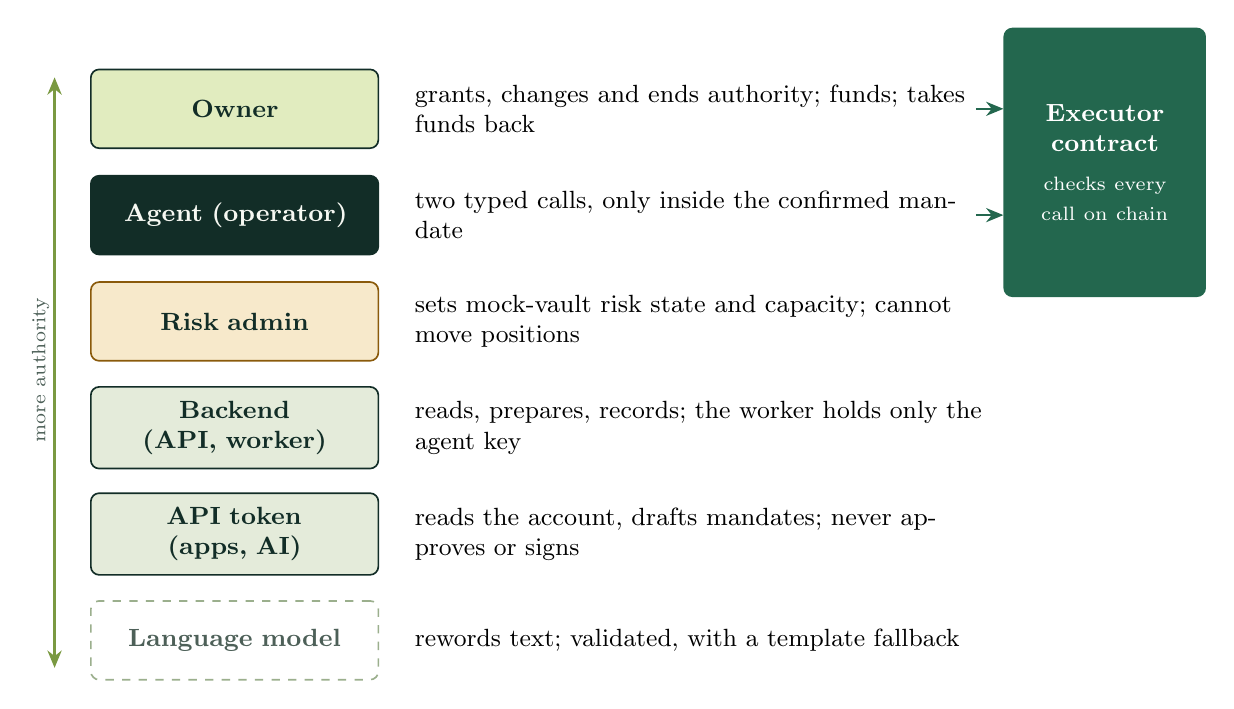
\begin{tikzpicture}[x=1cm,y=1cm]
  \foreach \y/\sty/\name/\can [count=\i] in {
    0/boxlime/Owner/{grants, changes and ends authority; funds; takes funds back},
    -1.35/boxdark/Agent (operator)/{two typed calls, only inside the confirmed mandate},
    -2.7/boxamber/Risk admin/{sets mock-vault risk state and capacity; cannot move positions},
    -4.05/boxsage/{Backend (API, worker)}/{reads, prepares, records; the worker holds only the agent key},
    -5.4/boxsage/{API token (apps, AI)}/{reads the account, drafts mandates; never approves or signs},
    -6.75/boxghost/Language model/{rewords text; validated, with a template fallback}}{
    \node[\sty,text width=3.3cm,minimum height=1.0cm,anchor=west] (t\i) at (0,\y) {\textbf{\name}};
    \node[anchor=west,text width=7.2cm,font=\small,align=left] at (4.0,\y) {\can};
  }
  \node[boxgreen,text width=2.2cm,minimum height=3.4cm,anchor=west] (exec) at (11.6,-0.68)
    {\textbf{Executor contract}\\[3pt]\scriptsize checks every call on chain};
  \draw[arr] (11.25,0) -- (exec.west |- 0,0);
  \draw[arr] (11.25,-1.35) -- (exec.west |- 0,-1.35);
  \draw[biarr,draw=bLime!70!bForest,line width=1pt] (-0.45,0.4) -- node[lblc,rotate=90,above=1pt]{more authority} (-0.45,-7.1);
\end{tikzpicture}
\caption{From most to least authority. Only the owner and the agent can change anything on chain, and the executor checks both.}
\end{figure}

\newpage
\subsection{Permission matrix}

\begin{btable}{@{}P{5.2cm}>{\centering\arraybackslash}p{1.25cm}>{\centering\arraybackslash}p{1.25cm}>{\centering\arraybackslash}p{1.25cm}>{\centering\arraybackslash}p{1.35cm}>{\centering\arraybackslash}p{1.25cm}>{\centering\arraybackslash}X@{}}
\headrow \thead{Action} & \thead{Owner} & \thead{Agent} & \thead{Risk admin} & \thead{Backend} & \thead{API token} & \thead{Model}\\ \midrule\endhead
Create executor, set mandate, fund & \yes & \no & \no & \no & \no & \no\\
Pause, resume, revoke & \yes & \no & \no & \no & \no & \no\\
Recover idle funds, withdraw a position to the owner & \yes & \no & \no & \no & \no & \no\\
\code{executeDeposit} / \code{executeWithdraw} within the mandate & \no & \yes & \no & \no & \no & \no\\
Send funds anywhere but the owner & \no & \no & \no & \no & \no & \no\\
Set a vault's risk state and capacity & \no & \no & \yes & \no & \no & \no\\
Approve a mandate draft (preview hash) & \yes & \no & \no & \no & \no & \no\\
Start a goal, answer questions, draft a mandate & \yes & \no & \no & \no & \yes & \no\\
Read the dashboard and activity & \yes & \no & \no & \no & \yes & \no\\
Mark a mandate \code{AUTHORIZED} (after chain checks) & \no & \no & \no & \yes & \no & \no\\
Choose questions, vault or limits & \no & \no & \no & \yes\textsuperscript{*} & \no & \no\\
Reword a question or summary & \no & \no & \no & \no & \no & \yes\\
\end{btable}
{\small\muted{\textsuperscript{*} Deterministic code (ACCE and the mandate builder); the owner reviews and approves the result.}\par}

\subsection{How each tier is implemented}

\begin{btable}{@{}P{2.6cm}P{6.3cm}L@{}}
\headrow \thead{Tier} & \thead{Enforced by} & \thead{Where}\\ \midrule\endhead
Owner & \code{onlyOwner} on every authority and recovery function; the owner is immutable per executor; withdrawals always pay the owner & \code{contracts/src/BoundraExecutor.sol}\\
Agent & Operator address, current version and nonce, fresh action ID, exclusive deadline, allowed vault and action, per-action and total caps, one allocation, lockup and expiry, no deposit into a degraded vault & \code{BoundraExecutor.sol} (\code{\_authorize}); checked again off chain by \code{prepareAction} and simulation\\
Risk admin & Vault owner only; changes risk flag and global capacity, never a position & \code{contracts/src/MockVault.sol}\\
Backend & No owner keys; worker modes (\code{observe\_only}, \code{monitor\_only}, \code{execute}); refuses an operator equal to the risk admin; reviewed manifest with pinned bytecode hashes & \code{apps/worker/src/runtime/activation.ts}, \code{packages/chain}\\
Browser session & SIWE bound to origin and chain, single-use nonce, \code{\_\_Host-} cookie (HttpOnly, Secure, SameSite=Strict), exact \code{Origin} and CSRF token on every change; owner always from the session & \code{apps/api/src/auth}\\
API token & Signed token statement decides the session kind; bearer only, never a cookie; admin routes refused; hashed, expiring, revocable from the app & \code{apps/api/src/auth}, \code{/app/connect}\\
Admin & Wallets in \code{ADMIN\_ADDRESSES}, browser session only & \code{apps/api/src/auth}\\
Language model & Output schema, same alternatives, no new numbers, vaults, addresses, links or guarantees; time and token budgets; template fallback & \code{packages/llm}\\
\end{btable}

\begin{keypoint}[Defence in depth]
Every agent action passes four gates: the deterministic policy, the off-chain chain guard (\code{prepareAction}), a simulation against current state, and the executor's own on-chain checks. Only the last one is trusted; the others fail early and explain.
\end{keypoint}

\section{Known-risk list}

Impact is rated for this testnet prototype; ``real funds'' marks risks that would be blocking before any mainnet use.

\begin{btable}{@{}>{\raggedright\arraybackslash}p{0.75cm}P{3.3cm}P{1.35cm}L P{3.4cm}@{}}
\headrow \thead{ID} & \thead{Risk} & \thead{Impact} & \thead{Mitigation in place} & \thead{Residual risk}\\ \midrule\endhead
R1 & Agent key stolen & \impact{High} & Bounded by the mandate: caps, one allocation, allowed vaults, withdrawals only to the owner. Separate account; owner can pause or revoke and recover funds. & Remaining budget can be used at an inconvenient time.\\
R2 & Server or hosting compromised & \impact{High} & No owner keys on the server; secrets are runtime settings only; agent key bounded as in R1; API tokens cannot move funds. & Misleading drafts are possible; the owner reviews the exact preview before approving.\\
R3 & Wrong agent decision & \impact{Medium} & Deterministic, tested policy; \code{prepareAction}, simulation and on-chain checks. & Caps limit harm but do not prove suitability.\\
R4 & Look-alike contracts or fake events & \impact{High} & Reviewed manifest with pinned runtime-bytecode hashes; risk events only from the two pinned vaults. & The manifest review itself is manual.\\
R5 & RPC provider fails or misreports & \impact{Medium} & Confirmation depth, block-hash checks, receipt re-checks; on failure the worker holds instead of acting. & A single public RPC is trusted; no second source.\\
R6 & Chain reorganisation & \impact{Low} & 5-block depth, 20-block scan overlap, terminal receipts re-checked for 20 blocks. & A deeper reorg forces a rescan.\\
R7 & Stuck or duplicated agent transaction & \impact{Medium} & Persist before broadcast, fenced leases, idempotent nonce reservations, identical-byte recovery, release after the deadline. & No automatic fee bumping.\\
R8 & Risk admin is a central fixture & \impact{Medium} & Can only set risk state and capacity; separate account from operator and deployer. & Not an oracle; stands in for real protocol signals.\\
R9 & Phishing or cross-site requests & \impact{Medium} & Origin-bound SIWE, \code{\_\_Host-} cookie, exact Origin and CSRF checks; wallet prompts show the real call. & Owners must still check the site address.\\
R10 & API token leaked & \impact{Medium} & Cannot approve, sign or move funds; hashed, expiring and revocable. & Can read the account and draft mandates until revoked.\\
R11 & Language model misleads & \impact{Low} & Wording only; validated; template fallback; labelled source. & None for authority.\\
R12 & Mock vaults and MockUSDC & \impact{Low} & Testnet only; principal 1:1; yields are labelled illustrative. & Real vault integrations need their own review (real funds).\\
R13 & No independent audit & \impact{High} & Unit, fuzz and stateful invariant tests; end-to-end runs. & Blocking before real funds.\\
R14 & Free hosting sleeps & \impact{Medium} & Health endpoints; the container restarts if any process stops. & The agent sleeps with the service; a paid plan or VPS removes this.\\
R15 & Stale screen invited repeated owner actions & \impact{Low} & Repeats were harmless on chain; the fix polls until the confirmed block and disables the controls meanwhile (PR \#11). & None once the fix is deployed.\\
R16 & Dependency supply chain & \impact{Medium} & Exact version pins, frozen lockfile, CI on every change. & No automated vulnerability scan yet.\\
R17 & Database lost & \impact{Low} & The chain is the source of truth for authority and funds; scheduled backups in the Compose stack. & Workflow history would be lost (Render's free database expires).\\
\end{btable}

\section{Evidence and next steps}

\begin{stable}{@{}P{5.0cm}L@{}}
\headrow \thead{Evidence} & \thead{What it covers}\\ \midrule
Contract tests (32, Foundry) & Owner-only changes, caps, lockup, replay, arbitrary-call denial, recovery; randomized invariants for budgets and principal.\\
API and worker integration (24, 29) & Sessions, tokens, owner isolation; leases, crash recovery, concurrency.\\
Browser suites (53 mocked, 2 real) & Every owner transaction, and the full journey with nothing mocked.\\
Base Sepolia run & Real owner and agent transactions; see the execution evidence report.\\
Public source verification & Every deployed contract matches the repository's source, checked by independent explorers (below).\\
\end{stable}

\subsection{Verified contract source}

Each deployed contract's source was published and verified against its on-chain bytecode, so anyone can read exactly what runs at the addresses in the reviewed manifest. This backs the bytecode comparison done before the manifest was pinned, and the mitigation of R4.

\begin{stable}{@{}P{3.1cm}P{7.2cm}L@{}}
\headrow \thead{Contract} & \thead{Address} & \thead{Verified on}\\ \midrule
MockUSDC & \href{https://base-sepolia.blockscout.com/address/0x13e7a4d02941a029Cf841f16E38eF377cb21e1Cf}{\texttt{\footnotesize 0x13e7a4d02941a029Cf841f16E38eF377cb21e1Cf}} & Blockscout\\
MockUSDCFaucet & \href{https://base-sepolia.blockscout.com/address/0xEbdc09B132066fF067E30FE077A58E818801FA2f}{\texttt{\footnotesize 0xEbdc09B132066fF067E30FE077A58E818801FA2f}} & Blockscout\\
LiquidVault & \href{https://base-sepolia.blockscout.com/address/0x7C0fC1a0551d5099d093E8D8b34a214758f7B27a}{\texttt{\footnotesize 0x7C0fC1a0551d5099d093E8D8b34a214758f7B27a}} & Blockscout\\
TimedVault & \href{https://repo.sourcify.dev/84532/0x7ffD08b7b52E26023142060D3f5dBDe27757CD84}{\texttt{\footnotesize 0x7ffD08b7b52E26023142060D3f5dBDe27757CD84}} & Sourcify, exact match\\
BoundraFactory & \href{https://repo.sourcify.dev/84532/0xFbD91368BfFA9AF5C7034bCB7F53Cc1eC906b7f4}{\texttt{\footnotesize 0xFbD91368BfFA9AF5C7034bCB7F53Cc1eC906b7f4}} & Sourcify, exact match; Blockscout\\
BoundraExecutor (the evidence run's) & \href{https://repo.sourcify.dev/84532/0x0e4c01b7fAc2e45a2a38eA7B9A0744D4eF0e9E2E}{\texttt{\footnotesize 0x0e4c01b7fAc2e45a2a38eA7B9A0744D4eF0e9E2E}} & Sourcify, exact match\\
\end{stable}
{\small\muted{An exact match means the deployed bytecode equals the compiled source including its compiler metadata. Verified with Foundry (\code{forge verify-contract}), Solidity 0.8.30.}\par}

\begin{note}[Before any real funds]
An independent audit of the contracts, a second RPC source, fee replacement for stuck transactions, real vault integrations with their own review, monitoring and alerts, and a legal review.
\end{note}

\end{document}
